\maketitle
%\thispagestyle{fancy}
\section{Introduction}

This is the full report.

\subsection{Goals}

The goals of this study were as follows:
\begin{enumerate}
  \item Establish a set of quantitative objectives for the Swarm revenue share allocation system.
  \item Evaluate to what extend the revenue sharing mechanism facilitates or impedes these objectives.
  \item Where suboptimal, propose alternative approaches or avenues of investigation that could improve the situation.
\end{enumerate}
Intermediate and side objectives were among the following:
\begin{enumerate}
  \item Describe plausible strategies in the revenue share acquisition game. Try to discover `bad' equilibria.
  \item Establish a market clearing model that includes a `quality' parameter tracking replication rate.
  \item Describe and evaluate alternative revenue sharing models.
\end{enumerate}

Due to time constraints, we only scratched the surface of the analysis of alternative revenue sharing models.

\subsection{Methodology}
%
Our basic approach was to produce a mathematical model of the Swarm economy that incorporates the details of `supply-side controls,' namely, the revenue sharing system.
%
We then evaluated our model against a list of general economic objectives of the system.\footnote{The objective functions discussed in the present report are quite different from the list initially reported in August and discussed with V.~Tr\'{o}n.
%
This change occurred because we discovered a way to derive the earlier objectives as intermediate targets from more fundamental --- and self-evident --- economic goals like growth and quality of service.}

More precisely, the logical (if not chronological) progression of our approach goes as follows:
\begin{enumerate}

  \item 
    Couch the Swarm network economy and its objectives in terms of a general microeconomic production model with objectives of demand, price, and `quality,' with the latter interpreted as replication rate.
    %
    As protocol designers, we would like to at least achieve a production vector on the efficient frontier of the production set.
  
  \item
    Introduce the notion of an abstract revenue sharing mechanism as a way to construct the feasible production set.
    %
    Efficiency of the resulting production vector then becomes a checkable condition on the revenue sharing mechanism.

  \item
    Identify an example of an efficient revenue sharing mechanism under idealised conditions.

  \item
    Describe the Swarm redistribution mechanism as part of a parametrised family (\S\ref{section:model}).
    %
    We look for conditions under which this implements an inefficient outcome using an agent-based approach.

  \item
    Describe the agent policy optimisation problem and establish classes of plausible policies (\S\ref{section:optimal}, \S\ref{section:risk}).
    %
    Observe which allocations (and reallocations) can result (\S\ref{section:feasible}).

  \item
    Discuss approaches to estimating or forecasting the unknown or random parameters in the model (\S\ref{section:estimation}).

\end{enumerate}

\subsection{System overview}

The Swarm Protocol is a decentralised storage service with blockchain-based payments and revenue sharing mechanism.
%
It comprises the following components:
%
\begin{enumerate}
  \item A peer-to-peer network of \emph{storage provider} nodes;
  \item A utility token, BZZ, deployed on an EVM chain (for mainnet Swarm, this chain is Ethereum mainnet);
  \item A system of 4 smart contracts that sell storage space on the (nodes participating in the) peer to peer network and redistribute the proceeds among the registered nodes.
\end{enumerate}
%
Two types of agents interact with the Swarm Protocol: users, a.k.a.~storage clients, who purchase storage quotas and upload and download data; and node operators (NOs), a.k.a.~storage providers, who provide their storage space and compute storage proofs in exchange for a share of the revenue.
%
It is also instructive to consider the Swarm system itself as a third (singleton) type of ``agent'' which intermediates between storage clients and storage providers.

For more details, see \cite{book-of-swarm}.

\subsubsection{Revenue sharing mechanism}

The topic of study of this report is the Swarm Protocol revenue sharing mechanism design and its effect on the overall system design objectives.
%
\begin{itemize}
  \item 
    The redistribution mechanism is governed by the Stake Registry and Redistribution contracts.
  \item 
    The network revenue is calculated by the Price Oracle (which gives the price) and Postage (giving the amount of storage consumed) contracts at each epoch.
    %
    The computation occurs when the Redistribution contract, triggered by a call to \code{claim()}, calls into the Postage contract to query the reward pot.
    %
    We treat these contracts largely as a black box (but see \S\ref{section:estimation}).
  
    \item 
    NOs may purchase \emph{shares} by calling the \code{stakeUpdate} function in the stake registry.
    %
    In the Book of Swarm and related literature, this operation is called \emph{depositing} or \emph{topping up stake}.
    %
    In this study, we prefer the term \emph{share} as we believe this gives a more accurate mental model of what entering into this position entails.

    Prior to SWIP-19, share balances were associated to an overlay address.
    %
    Post SWIP-19, balances are associated to a Gnosis chain address together with a derived overlay address.
    %
    That is, after these changes, each Gnosis chain address is associated to a unique share balance, instead of possibly several keyed by different overlay addresses derived using different nonces.

  \item
    Prior to SWIP-20, shares were priced at a static value $1$.\footnote{Except for integer division problems, the price could be replaced by any constant number without affecting the model.
    %
    The convention $p=1$ matches how balances were tracked in the stake registry implementation prior to version 0.9.1.}
    %
    Post SWIP-20, the price is the per-chunk storage price as given by the price oracle for that epoch.

  \item
    Nodes are divided up into \emph{replication neighbourhoods} or \emph{bins} according to the first $D$ bits of their overlay address, where $D$ is a number determined locally by the amount of data being stored on the platform.
    %
    At time of writing, $D=11$.
    %
    Since in this study, we will assume that $D$ is a global constant, we don't need to go into details of what happens when $D$ changes.

  \item
    Time is divided into \emph{rounds} or \emph{epochs} of 152 Gnosis chain blocks --- targeting 12 minutes 40 seconds.
    %
    Each epoch, a bin is selected uniformly at random.
    %
    NOs belonging to that bin may participate in the revenue sharing system during that epoch if they satisfy a few additional conditions:
    \begin{enumerate}
      \item They have not purchased additional shares within the past 2 epochs.
      \item They are not \emph{frozen} as a penalty for a consensus fault. Freezing penalties last for about 1 day.
      \item They have shares in excess of a minimum threshold $\tau$. For the versions under consideration in this study, $\tau=10$ BZZ.
    \end{enumerate}

  \item
    To participate in the revenue sharing system, nodes must submit storage proofs during a \emph{commit} and \emph{reveal} phases (the first and second quarters of an epoch --- 38 blocks, or 3 minutes 10 seconds each).
    %
    Commits are checked for agreement in a rudimentary consensus system.
    
    In the final \emph{claim} phase, any entity can call the \code{claim()} function of the redistribution contract.
    %
    This function randomly selects a node from among those that successfully submitted a commit and reveal in the previous phases, with probability weighted by the share balance of that node.
    %
    The selected node receives the full network reward for that round, paid out from the Postage contract.

  \item
    Network revenue and share prices are both denominated in BZZ tokens.

\end{itemize}

\subsubsection{Scope}
\label{section:scope}

In our study, we focus only on the revenue share redistribution mechanism that governs the relationship between storage providers and the Swarm system.
%
The demand-side part of the relationship, governing the relationship between storage clients and the Swarm system, is out of scope.


\paragraph{Versions}
Our study is based on version 0.8.6 of the storage incentives contracts.
%
Since this version only introduced an update to the redistribution contract that is out of scope of the model, our model applies equally well to the versions of contracts deployed at version 0.6.0 (or version 0.4.0 in the case of the stake registry).


\subsection{Recommendations}

\begin{enumerate}
  \item
    As the network grows into the petabyte range, small NO operations such as a single laptop become unviable because of risk of ruin.
    %
    If demand for Swarm revenue share remains robust, the emergence of stake pools or liquid stake solutions is inevitable.

    The Swarm community should consider what staking pools might look like and whether the core protocol should be changed to either directly support stake pools or facilitate community-led initiatives.

  \item
    We have found theoretical aggressive share minting strategies that lead to stagnant stake allocations that are problematic from an efficiency perspective.
    %
    Empirically, no one is currently pursuing such strategies, but the situation should be carefully monitored.

  \item
    The lack of options to reallocate stake is a potential barrier to economic efficiency and hence optimal pricing.
    %
    The Swarm Protocol designers should consider introducing more reallocation opportunities so that they have an opportunity to undergo real price discovery.
    %
    However, care should be taken to ensure that revenue share does not flow too readily to the the agent with lowest costs, giving it market power.

  \item
    The Swarm community should consider how it wishes to prioritise the tradeoff between replication rate (and other QoS) targets and growth targets (realised demand and revenue).

\end{enumerate}



\newpage
%%%%%%%%%%%%%%%%%%%%%%%%%%%%%%%%%%%%%%%%%%%%%%%%%%%%%%%%%%%%%%%%%%%%%%%%%%%%%%%

\section{Objectives of the system design}

\begin{notes}

  \item The fundamental goal of the revenue sharing system is to entice node operators to provide a storage service that meets demand and quality of service (QoS) targets.

  Unfortunately, Swarm faces a difficulty in directly measuring the amount or quality of service provided by NOs; specifically, such measurement is vulnerable to a \emph{deduplication attack} where nodes claim to be hosting multiple replicas of the same data when in fact they only store one.
  %
  Therefore a supplementary approach to revenue share allocation is used to remove an incentive to falsely inflate storage capacity.

  \item This directly entails three directly measurable dimensions of objectives: realised demand, protocol revenue, and QoS in the form of replication rate.

  \item In \S\ref{section:efficiency} we define and establish equivalent conditions for Pareto optimality of a (demand, price, QoS) outcome.

  \item In \S\ref{section:redistribution} we discuss redistribution mechanisms that achieve Pareto optimal outcomes (given fixed exogenous demand surface) and pose the question of whether Swarm's system is one of them.

  \item In \S\ref{section:decentralization} we consider measurement of decentralisation on various axes and its relation to monopoly control of allocation, particularly censorship, and pricing.

  \item Yet another, rather more specific, goal of the redistribution system is to guarantee consistency of the chunk index. Do we consider this a type of QoS guarantee? Either way, it is somewhat outside the scope of our models.

\end{notes}

\subsection{Objective functions}

We identify three measurable core objective functions that exhibit the economic performance of the Swarm network:
%
\begin{enumerate}

  \item Protocol revenue, i.e.~the total cash flows into the Postage contract;

  \item Realised demand, i.e.~the total amount of storage quotas purchased from the Postage contract;

  \item Apparent replication rate, i.e.~the (mean) number of distinct nodes producing successful proofs in the redistribution game each round.\footnote{As discussed above, the true replication rate could be lower than the apparent replication rate because of deduplication/compression.}

\end{enumerate}
%
The target of the revenue and demand objectives is straightforward: the higher the better.

\subsubsection{Protocol revenue}

It might also be reasonable to consider the total \emph{profit} of NOs as an objective, but this is not directly measurable.
%
Similarly, protocol profit, if there were any part of revenue claimed by the protocol, would also be a reasonable objective.

Aggregate NO cost minimisation is still required for these objectives, but the savings are not necessarily fully communicated to users in the form of price reductions.


\subsubsection{Realised demand}

Straightforward.
%
We note that under the demand theory of ordinary goods, demand decreases with price (given fixed QoS).
%
Similarly, it is reasonable to assume that demand increases with QoS.
%
So this objective is related to the objective of minimising price at a given QoS, or maximising QoS at a given price.

\subsubsection{Quality of service}

The stated goal of the Swarm Protocol design is to target a replication rate of 4.
%
We argue that a replication rate of higher than 4 would not be objectionable if it did not negatively impact the other two objectives.
%
Thus replication rate is also a function that we wish to maximise as part of a multi-objective optimisation framework.

In our model of the Swarm storage service, nodes are simply either active or inactive --- for simplicity, we are not taking into account any gradations in service quality (such as retrieval latency and bandwidth).

\subsection{Efficiency}
\label{section:efficiency}

Broadly speaking, economic efficiency means that resources are allocated where they can be deployed most productively.
%
That is, efficient allocations are those that optimise economic growth.

%The Swarm network maintains an internal state that controls the distribution of revenue for the storage service; this redistribution is efficient if it is optimised for growth of the demand serviced, given fixed exogenous world state and constraints on the quality of service --- most essentially for us, the replication rate $q\geq 4$.
%
%All other things being equal, demand tends higher when prices are lower, so an equivalent goal is the optimisation of price at the target replication rate.


%
%An efficient allocation of Swarm revenue share would allow the NOs with lowest costs to become active, driving those with higher costs out of business and allowing the cost savings to be passed onto customers in the form of lower price per replica.



\paragraph{Market clearing model} This is really somewhat incidental to the discussion of revenue redistribution, so we will treat it only briefly. See \cite[\S10]{mascollel1995microeconomic}.

If we write $\mathcal{D}=\uR$ for demand space, $\mathcal{P}=\uR$ for price space, and $\mathcal{Q}=\uR$ for QoS (replication rate) space, then the Swarm protocol rules and exogenous world state determines a set of feasible allocations
%
\[
  X \subset \mathcal{D}\times\mathcal{P}\times\mathcal{Q}.
\]
%
Here, a point $(D,p,q)$ is \emph{feasible} if:
\begin{itemize}
  \item The aggregate demand $D$ is realisable at price $p$ and QoS $q$;
  \item The realised revenue $R=pD$ can be distributed among a population of storage providers \emph{in some way} such that they would collectively be prepared to meet the demand $D$ with replication rate $q$, i.e.~provide $qD$ units of storage.
\end{itemize}
%
Since our focus is revenue redistribution, we black box the demand surface $X(p,q)$ as an exogenous signal.
%
The means by which the supply-side revenue distribution is achieved is within the purview of the Swarm protocol designers.

\begin{definition}[Pareto efficiency]

  The market state $(D,p,q)$ is \emph{(Pareto) efficient} if the following equivalent conditions are satisfied:
  \begin{enumerate}
    \item $p$ is minimal in $X_q$;
    \item $q$ is minimal in $X_p$;
  \end{enumerate}

\end{definition}

If Swarm storage is an ordinary good, for any $q\in \mathcal{Q}$, the feasible slice 
\[
  X_q = X \cap (\mathcal{D}\times\mathcal{P}\times\{q\})
\]
is a downward-sloping curve in the positive quadrant $\uR^2$.\footnote{The reasoning is as follows: The Walrasian budget set of consumers is monotone decreasing in $p$, hence the solution of the UMP is decreasing in the amount of Swarm storage consumed.}
%
That is, the storage price is minimised within the feasible region if and only if demand is maximised, so objectives (1) and (2) are equivalent.

\paragraph{Price optimisation}
To transform this optimisation problem into a \emph{price taker} problem where $p$ is given and $q$ may vary, as in objective (3), we look for a selection rule 
\[
  \xi^*:\mathcal{P}\rightarrow X\cup\{\bot\}
\]
that assigns a feasible state $\xi^*(p)=(D^*,p,q^*)\in X\cap \mathcal{D}\times\{p\}\times\mathcal{Q}$ such that $q^*$ is maximal in $X\cap \mathcal{D}\times\{p\}\times\mathcal{Q}$.
%
Classical supply theory tells us that $q^*(p)$ is \emph{increasing} in $p$. 
%
Then the price objective can be achieved by finding the minimal $p$ such that $q^*(p)\geq 4$; if $q^*$ is strictly increasing in $p$, continuous, and $q^*(0)=0$, then this minimum achieves the target rate $q^*=4$.


\subsection{Redistribution mechanisms}

\label{section:redistribution}

The mechanism design approach to economic allocation tells us to search for a budget-balanced redistribution mechanism
\[
  \mathbf{M}:\uR \times \Omega \rightarrow \uR^\Overlay
\],
specifying the amount $\mathbf{M}(R,\xi)_a$ each address $a\in\Overlay$ receives based on the total revenue $R\in\uR$ and some internal state vector $\xi\in\Omega$, together with a (Bayes-Nash) equilibrium $\xi^*(R)\in\Omega$.

The endogenous state space can take several forms, but we ask that it at least record whether each node is \emph{active} via a map $\mathtt{on}:\Omega\rightarrow \{\bot,\top\}^\Overlay$.
%
Then we can define the \emph{replication rate} of the equilibrium $\xi^*$ by the formula
\[
  q(\xi^*) = \sum\mathtt{on}(\xi^*);
\]
say also that $(\mathbf{M},\xi^*)$ \emph{implements} $q$.

\begin{example}[Swarm incentives v0.4.0]
  
  In the version of the Swarm mechanism under consideration, the endogenous state vector $\xi^*$ consists of a mapping $(\mathtt{on},x):\Overlay\rightarrow \{\bot,\top\}\times\uR$ that identifies whether a node is active and what their equity balance is.

\end{example}

\begin{example}[Equal weighting]

  Assume equal stake distribution $\xi \equiv 1$ and let $S(p)=S(p,\mathbf{1})$.
  %
  If the replication rate is $q$, then each individual agent supplies $S(p)/q$ units of storage, and the total number of distinct units of data that can be stored at replication rate $q$ is $S(p)/q$.
  %
  Thus, the microeconomic equilibrium equation is $D(p,q)=S(p)/q$.
  %
  It has one degree of freedom.

  In the presence of dynamic NO populations, and especially without Sybil resistance, equal weighting is not a reasonable approach to redistribution: it is better to assume the population of potential NOs is very large, and that almost all nodes have zero or very small weight.

\end{example}

\paragraph{Identifying an optimal allocation}
Suppose we have access to the variable costs $O:\Overlay\rightarrow\uR$ of each NO, that is, the cost of providing a single active node.
%
For simplicity, we assume that $O$ does not depend on the quantity of storage provided; this is not as ridiculous as it sounds if we assume that NOs must reserve a certain amount of computation to run their node, regardless of how full the reserve is, and that realised demand does not stray past a power of two, triggering a neighbourhood split.
%
Finally, we assume that $\Overlay\subseteq\N$ is well-ordered and that $O(a)$ is increasing in $a$, i.e.~the node addresses are sorted in order of increasing operating cost.

The following result is not hard to prove:
%
\begin{proposition*}
  Under the above assumptions, let $K\in\Overlay$ be the maximum index such that
  \[
    \sum_{k=0}^KO(k) \leq R.
  \]
  Then the redistribution weights
  \[
    w_k = \left\{ \begin{array}{ll}
      O(k)/\sum_{i=0}^KO(i) & k\leq K \\
      0 & k > K
    \end{array} \right.
  \]
  define a QoS-optimal allocation with replication rate $K$.
\end{proposition*}

The Swarm protocol does not have direct access to the quantities $O(a)$, so the preceding mechanism cannot be implemented as stated.
%
Instead, we must rely on the laws of competition to induce rellocation of market share to the NOs with lowest costs.

\begin{question} Does the Swarm redistribution mechanism implement $(p^*(4),4)$? \end{question}

\subsection{Tokenisation}

In this section, we establish trade ranges in a setting where equity positions are tokenised and freely tradable.

\begin{itemize}

  \item The space of revenue share allocations state space is the cone $\uR^K$, where $K$ is the number of (potential) stakeholders.

  \item There's a projection $\uR^K\setminus\{0\}\rightarrow \Delta^{K-1}$ onto the set of allocations; payoffs of a stake position depend only on the quotient.

  \item Suppose NOs can buy and sell equity stakes in arbitrary quantities. 
  %
  It is rational for an active NO $i$ to accept a one-off payment $P$ for an amount $k$ of stake if 
  \[
    \frac{S_i}{\sum S} R - O_i \leq P + \max\{ \frac{S_i-k}{\sum S} R - O_i, 0\}
  \]
  with the understanding that $i$ will shut down their node if $\frac{S_i-k}{\sum S}R<O_i$.
  %
  In other words, the acceptance threshold is
  \[
    P \geq \min\left\{ \frac{k}{\sum S} R, \frac{S_i}{\sum S} R - O_i \right\}
  \]

  \item Meanwhile, it is rational for an active NO to offer a payment $P$ for $k$ shares if
  \[
    P \leq \frac{k}{\sum S}R.
  \]
  For an inactive NO with operating cost $O_i$, the figure is
  \[
    P \leq \frac{k}{\sum S}R - O_i.
  \]

  \item Clearly, a trade is therefore possible if the buyer is either already active, or is inactive but with lower operating cost than the seller.
  %
  We can therefore expect a trend towards consolidation and stake accumulation towards NOs with lower operating costs.
  
  If $i^*$ is the index maximising $O_i/S_i$, then the price (per unit share) interval in which trading is possible is
  \[
    \left[ R/\sum S - O_{i^*}/S_{i^*}, \min\{ R/\sum S, p_{\oracle} \} \right]
  \]

\end{itemize}

\begin{proposition*}

  Suppose that revenue share allocations are tokenised and freely tradable in any quantity.
  %
  Then from any starting allocation, there exists a sequence of incentive-compatible trades that result in the optimal allocation of Proposition \ref{section:efficiency}.

\end{proposition*}

This argument assumed that the forecast returns $R$ do not depend on whether or not the trade occurs. 
%
But a buyout of an active node by another active node could cause the observed replication rate to go down, causing the quoted storage price to go up. 
%
Under this condition, a sophisticated NO would revise their forecast for $R$ --- broadly speaking, the effect should be to drive revenue up in the short term (particularly for existing storage quotas, which cannot be cancelled), but to drive demand down in the medium term.

(Of course, the buyer could also assign the stake to a new address that runs on deduplicated storage, preventing a reaction by the price oracle.)


\subsection{Decentralisation}
\label{section:decentralization}

Decentralisation is usually a primary objective of blockchain-based services.
%
Decentralisation can be measured in terms of the difficulty by which an adversary can unilaterally control aspects of the system.
%
In the context of Swarm, we argue that the primary vectors of centralisation with which the system designer should concern himself are:
%
\begin{enumerate}
  \item Censorship power, an aspect of allocation (i.e.~whether or not to provide the service for a given offer);
  \item Market power, which can lead to monopoly pricing.
\end{enumerate}

Generally we would like to compute concentration or dispersion of some distributions of nodes by controlling entity.
%
Because node addresses are easily Sybilled, we should take some care about how we define the domain of such distributions.
%
A sophisticated approach based on linking and labelling addresses by owner is possible and has been applied with success across the blockchain industry \cite{}, though error-prone \cite{}.

\begin{example}[Concentration measures]
  
  In US anti-trust legislation, the Herfindahl-Hirschman index ($L^2$ norm) is used as a measure of concentration.
  %
  We advocate the use of Shannon entropy because of its composition rule.

\end{example}

\subsubsection{Censorship}

Data uploaded to the Swarm network is chunked and spread, essentially uniformly at random, across a number of replication bins that scales with the data size.
%
An entity that controls one of these replication bins can choose not to store or serve chunks of certain uploads that would land in its bin.
%
For some types of data, for example encrypted blocks, loss of a single chunk is as good as loss of the complete data; this therefore gives the controlling entity censorship power over such data.

The simplest measure of control in a given replication bin is the number of active nodes participating in revenue sharing; a higher number indicates greater decentralisation.
%
This number is analogous to the \emph{Nakamoto coefficient} used to measure failure-resistance of Bitcoin consensus.

A more refined approach would measure the ability of a single entity to (probabilistically) gain control over the replication bin's consensus over the chunk index; this ability scales with the equity share of the entity within that bin (and hence probability to be selected as consensus leader on any given cycle).

A highly concentrated equity pool may also indicate a trend towards consolidation and hence reduced replication rate. 
%
If equity is allocated efficiently, this may also give an indication of differing operating costs.

\subsubsection{Pricing power}
%
In order to gain pricing power over the Swarm protocol, an entity must have sufficient market share to directly influence either the BZZ/USD price or the price oracle.
%
The price oracle can be influenced by manipulating the replication rate.

To be able to influence the global replication rate with any degree of reliability, the adversary likely controls nodes across many replication bins.
%
Since such nodes necessarily have different Ethereum addresses (post SWIP-19), the assumption of one address per entity won't hold for measuring this; we must link addresses together.

If the monopolist manages to acquire enough equity to make entry unprofitable, he can achieve this, especially if reallocations of stake between nodes is possible.

\subsubsection{Neighbourhood weight}

We expect equity to be balanced across neighbourhoods in equilibrium, since all neighbourhoods have equal earning potential.
%
However, in practice non-uniform distributions arise; these could be understood as an indicator of allocative inefficiency.
%
Currently, the only opportunities for rebalancing investment across replication neighbourhoods are:
\begin{enumerate}
  \item Minting new shares in under-invested neighbourhoods;
  \item Switching off nodes in over-invested neighbourhoods;
  \item Under SWIP-19, moving a node from an over-invested neighbourhood to an under-invested one.
\end{enumerate}
%
The dispersion of neighbourhood weights is a measure of how well these moves permit a convergence on balanced equity.


\newpage
%%%%%%%%%%%%%%%%%%%%%%%%%%%%%%%%%%%%%%%%%%%%%%%%%%%%%%%%%%%%%%%%%%%%%%%%%%%%%%%

\section{Incentive model}
\label{section:model}

\begin{notes}
  
  \item We begin by establishing the incentive model for node agents and writing the policy optimisation problem in a general form.

  \item We also exhibit the most basic rationality constraint for agent policies, that of \emph{rational liveness} --- an NO will not activate their node in a given epoch unless it is profitable to do so.

  \item Assumptions of the model are delineated.

\end{notes}
\subsection{Preliminaries}

\paragraph{Addresses}

The set of agents is denoted $\Overlay$.
%
It can be realised as a set of \emph{overlay addresses}, for example, $\Overlay \cong \mathbb{F}_2^{256}$.

The set of overlay addresses is divided into a set $\Bins$ of \emph{bins}.
%
In \cite{book-of-swarm}, these are also called \emph{neighbourhoods}; we prefer the term `bins' because neighbourhoods can also be of various different sizes.
%
We are given a surjective map $\bin:\Overlay\rightarrow\Bins$ that takes an overlay address to the bin to which it belongs.
%
The fibre of $\bin$ over a bin $\nu\in\Bins$ is denoted $\Overlay_\nu$.

In deployments, we have $\Bins\cong \mathbb{F}_2^D$ and the function $\bin$ is projection on the first $D$ bits, where $D$ is a network-wide dynamic variable called the \emph{network (log-)radius}.
%
For any $\nu\in\Bins$, we can then identify $\Overlay_\nu\simeq\mathbb{F}_2^{256-D}$ by projecting out the first $D$ bits.


\paragraph{Balances}
\begin{itemize}
  \item 
    Write $\uR := [0,\infty)$. Except when otherwise indicated, we consider it equipped with Lebesgue measure.

\end{itemize}

\paragraph{Summation}

Fix the following notation:
\begin{itemize}
  \item if $x\in \mathbb{R}^I$ is a vector of finite length, write $\sum:=\sum_I:\R^I\rightarrow\R$ for the sum of the coordinates. On $\uR^I$ this coincides with the 1-norm.
  \item If $J\subseteq I$ is a subset, write $\sum_J$ for the composite $\R^I\stackrel{\pi_J}{\rightarrow}\R^J\stackrel{\sum}{\rightarrow}\R$, that is, summation over the coordinates in $J$.
  \item If $i\in I$ is a single element, write also $\sum_{\hat{i}}$ as a shorthand for $\sum_{I\setminus\{i\}}$.
  \item If $M\leq N$ are natural numbers and $x\in\R^{\Overlay\times N}$, write $x_{\leq M}\in \uR^{\Overlay\times M}$ for the projection on the first $M$ terms.
\end{itemize}

\paragraph{Weighting functions}

\begin{definition}

  A \emph{weighting function} on a stake registry $\uR^N\setminus\{0\}$ is a measurable function $w:\uR^N\rightarrow[0,1]^N$ such that $\sum w(\vec{s}) \leq 1$ for all $\vec{s}\in \uR^N$.
  %
  A weighting function is \emph{complete} if in fact $\sum w(s) = 1$ for all $s\in \uR^N$.

\end{definition}

\begin{example}[Even weighting]
  \emph{Even weighting} is the complete weighting function $w(s) = s/\sum s$.
\end{example}


\begin{example}[Adjusted shares]

  Suppose given an \emph{adjustment} function $g:\uR\rightarrow\uR$. 
  %
  Applying it to each coordinate gives a function
  %
  Then the \emph{adjusted} even weighting function is defined $w(s) = g(s)/\sum g(s)$.

\end{example}

\begin{example}[Entry threshold]
  For any $\tau\in\uR$, we can define a ``gate'' function by
  \[
    g_\tau(r) := \left\{\begin{array}{ll} 0 & r<\tau \\ r & r\geq\tau\end{array}\right.
  \]
\end{example}

For each $i\in I$, observe that
\[
  w_i(s) = 1 - \frac{\sum_{I\setminus\{i\}}g(s)}{\sum_I g(s)}
\]
so that
\begin{align*}
  \frac{\partial w_i}{\partial s_i}(s) &= g'(s_i)\cdot \frac{\sum_{I\setminus\{i\}}g(s)}{(\sum_I g(s))^2} \\
  &=g'(s_i)\cdot\left[ \frac{1}{\sum_I g(s)} - \frac{g(s_i)}{(\sum_I g(s))^2} \right].
\end{align*}

To see what's going on here, set $g(s)\equiv s$; the terms are then
\[
  \frac{\partial w_i}{\partial s_i}(s)=
  \underbrace{\frac{1}{\sum_I s}}_{\text{issued share}} - \underbrace{\frac{s_i}{(\sum_I s)^2}}_{\text{dilution}} .
\]
Clearly, the value of the newly issued share is independent of the initial share, while the effect of dilution is greater when the initial share is greater.

\begin{lemma}

  Let $U\subset \uR^N\setminus\{0\}$ be open and suppose that $g$ is differentiable and concave on $U$.
  %
  Then the even weighting function $w_g := g(s)/\sum g(s)$ is concave on $U$.

\end{lemma}
%
\begin{proof}

  By the formula expressed above, $\partial w_i/\partial s_i(s)$ is monotone decreasing as long as $g'(s_i)$ is. \qedhere

\end{proof}

\subsection{State and environment}

Each agent is considered to run two accounts: cash and equity (i.e.~stake).
%
The state space for each agent $a$ is therefore $\Xi_a\simeq\uR^2$.
%
Of these, only the equity is explicitly registered in a Swarm contract, namely, the stake registry.
%
We distinguish the stake registry state as $\Xi_S$.
%
The cash balance is an abstraction; it can be estimated in practice as the balance of an Ethereum address associated to the target agent's overlay address.\footnote{The deployed stake registry also records the block number of the most recent update to each equity account. This is used to prevent revenue share being claimed during the delay period --- currently 2 epochs --- immediately following an update.}

We also introduce a sample space $\Env$ of \emph{environment state} that may record information about demand on the Swarm network, signals coming from external markets, and preferences of the agents.
%
We endow the environment with a filtered $\sigma$-algebra $\{\mathcal{F}_t\}_{t\in\N}$, so that we can make sense of the expected values $\Expectation_t[\tilde{X}]$ of random variables defined on $\Env$ at time $t$.
%
It supports a number of processes that NOs need to use
\begin{itemize}
  \item The \emph{network revenue} $\tilde{R}_t\in \uR$.
  \item The \emph{(variable) operating cost} $\tilde{O}_{a,t}\in\uR$ of agent $a\in\Overlay$.
  \item If the network revenue is denominated in a different currency than the num\'eraire (e.g.~revenue denominated in BZZ with a USD num\'eraire), we should also track the corresponding price process $\tilde p_\mathrm{BZZ}^\mathrm{USD}$.
  \item The share price process $\tilde{p}_{S,t}$.
\end{itemize}
Note that we use tildes to denote random variables.
%
The environment also includes information about the preferences and policies of other agents.

Our interpretation of the filtered $\sigma$-algebra is that the $(\Env,\mathcal{F}_t)$-measurable functions represent the observable world at the \emph{end} of the $t$th epoch when revenue, operating costs, and the actions of other agents are realised.
%
Decisions about the $t$th epoch are made at the \emph{beginning} of the epoch, so must be made on the basis of the expectation operator $\Expectation_{t-1}$ from the previous epoch.

\paragraph{Epoch length}
%
The epoch for the purposes of policy formation need not be tied to the length of the Swarm Protocol round (i.e.~152 blocks).
%
In practice it may be much longer; for example, NOs may decide to turn their nodes on or off on a daily or longer timeframe.

\paragraph{Time summation}
%
The discounted sum of a real-valued process $\tilde{X}_n$ with discount rate $r>0$ is defined as
\[
  \sum_{n\in\N}(1-r)^n\Expectation_0[\tilde{X}_n],
\]
where expectation is taken with respect to the information $\mathcal{F}_0$ available at the reference time $0$.
%
If $\tilde{X}_n$ is a martingale, we have $\Expectation_0[\tilde{X}_n]=X_0$ (the latter is known at time $0$), and the discounted sum simplifies to 
\[
  \sum_{n\in\N} (1-r)^n X_0 = rX_0.
\]

\paragraph{Cash flow}
A state $(\xi_S,\omega)\in\Xi_S\times \Env$ is \emph{expected cash-flow positive} for agent $a$ at time $t$ if 
\[
  \Expectation_t[w_a(\tilde S_{t+1})\cdot \tilde{R}_{t+1}] \geq \Expectation_t[ \tilde{O}_{a,t+1} ];
\]
that is, if the agent makes money in expectation if he turns on his node during epoch $t+1$.

  
The full state space of the system is therefore $\widehat{\Env}:=\prod_{a\in\Overlay}\Xi_a\times \Env = \Xi_S\times\Xi_C\times\Env$.

\subsection{Actions}

At each epoch, a node operator makes three choices:
%
\begin{itemize}
  \item Mint a number $x\in\R$ of new shares at the current oracle price $p_S$.
  \item \emph{Cash out} an amount $y\in\uR$ as utility.
  \item Either be \emph{active}, i.e.~provide the storage service, or be \emph{inactive}.
\end{itemize}
%
The amounts transferred must be \emph{within budget} in that $p_Sx+y\leq \xi_\mathtt{cash}$ where $\xi_\mathtt{cash}$ is the current balance of the cash account.
%
That is, the space of actions given balances $\xi_a=(\xi_\mathtt{cash},\xi_\mathtt{eq})\in\Xi_a$ is
\[
  \actions(\xi_\mathtt{cash},\xi_\mathtt{eq}) = \{(x,y)\in \uR^2 \mid p_Sx+y\leq \xi_\mathtt{cash} \}
\]
%
If $x+y = \xi_\mathtt{cash}$, we say the move is \emph{budget balanced}.

We hence represent action as a vector
\[
  s = (s_\mathtt{mint},s_\mathtt{div},s_\mathtt{on}) \in \uR \times \uR \times \{1,0\}.
\]

\subsection{State transition}
The transition formula for the local state $\Xi_a$ is given by:
\[
  (s_a; (\xi_\mathtt{cash},\xi_\mathtt{eq})) \mapsto
    (\xi_\mathtt{cash}-p_Ss_\mathtt{mint} - s_\mathtt{div} + s_\mathtt{on}\cdot (w_i(\tilde{\xi}_\mathtt{eq})\cdot R(\tilde\omega) - O_a(\tilde\omega)), \xi_\mathtt{eq} + s_\mathtt{mint}).
\]
The actions of other agents affect the local state $\xi_a$ of agent $a$ only through their effect on $w_i(\tilde{\xi}_\mathtt{eq})$, and that only if $a$ is active through that round.

Note that the action $s_a$ of agent $a$ completely determines the state transition of its equity account, and the actions of all agents completely determine the stake registry update $\Xi_S$.


\subsection{Policies}

A \emph{policy} is a function $\pi:\widehat{\Env}\rightarrow\actions$ such that $\pi(\xi,\omega)\in\actions(\xi)$ for all $(\xi,\omega)\in\widehat{\Env}$.
%
That is, it is a rule for what to do in each environment state.
%
Rational, sophisticated NOs will seek optimal policies.

A policy is \emph{budget balanced} if every action it recommends is budget balanced.
%
For fixed $\omega$ and starting state $\xi$, a budget balanced policy is determined by a single number $\pi(\xi,\omega)_\mathtt{mint}\in\uR$.

\paragraph{Passive policies}
%
A \emph{passive policy} is one which never buys new shares; that is, $\pi(\hat\xi)_\mathtt{mint}=0$ for all $\hat\xi\in\widehat{\Env}$.
%
A budget-balanced passive policy cashes out the entire cash balance on every turn. 
%
That is, $\pi(\hat\xi)_\mathtt{div}=\hat\xi_\mathtt{cash}$ for all $\xi$.

Passive policies form a reasonable starting point for iterative approximation schemes to optimal policies.
%
Moreover, empirically speaking, nearly all NOs in the current Swarm network follow a passive policy.

If $i$ adopts a passive policy, $w_{i,t}$ is always monotone decreasing in time; i.e.~agent $i$'s equity share can only decrease over time.

\paragraph{Rational liveness}
%
A policy obeys \emph{rational liveness} if 
\[
  \pi(\xi)_\mathtt{on} = \top \qquad \Leftrightarrow \qquad \xi\text{ is expected cash-flow positive}.
\]
That is, a policy obeys rational liveness if the operator turns on the node if and only if it would be expected cash-flow positive to do so.

\paragraph{Value function}
The \emph{value function} of a policy $\pi$ with starting state $(\xi_0,\omega_0)$ is
\[
  V_\pi(\xi_0,\omega_0) = \sum_{n=0}^\infty (1-r)^n\Expectation_0 \left[ (\tilde{\xi}_n)_\mathtt{div} \mid \xi_{<n}, \omega_{<n}\right].
\]


\subsection{Assumptions}

We summarise here the intuitive sense of the assumptions implicit in this model and comment on how important they are.

\begin{enumerate}
  \item \emph{Stake update cool-off}. %
    We assume that NOs may \code{commit()} and receive revenue in the same epoch that they make a stake update.
    %
    However, in the actual redistribution contract, \code{commit()} reverts if fewer than two rounds have passed since the most recent update.\footnote{\url{https://github.com/ethersphere/storage-incentives/blob/v0.9.1/src/Redistribution.sol\#L304-L306}}
    %
    This discrepancy is not serious if we assume agents make decisions on a much longer timescale than 152-block rounds, for example daily.

  \item \emph{Storage service quality}. %
    We assume that the Swarm protocol is able to detect whether or not the storage service is provided and that a node is eligible for payouts if and only if it is active.
    %
    There are no gradations of service quality for a single node.
    %
    It follows that during each epoch, each NO may choose between providing the service or not providing it; there are no third options where the system can be `fooled' into paying out a reward where there is no service.
    
    We also assume that whenever the service is on, the NO remains in consensus with the rest of the neighbourhood; that is, slashing over safety failures is not considered.
    %
    This assumption is what makes the changes in the v0.8.6 upgrade of the storage incentives out of scope.

  \item \emph{Single node}.
    %
    We assume each agent operates at most one node.
    %
    Equivalently, agents may operate multiple nodes, but policies for each node are decided independently and costs scale linearly.
    %
    In particular, we do not consider the possibility of running a \emph{deduplication attack}, where an NO can run multiple nodes that share exactly the same storage backend.

  \item \emph{Common knowledge}.
    %
    The distribution of the revenue process $\tilde{R}_t$ is known to all participants.

  \item \emph{Independence}.
    %
    The revenue and operator cost processes are independent of the internal state $\Xi$.
    %
    In particular, no agent's actions affect the outcomes of these processes.

  \item \emph{Static neighbourhood set}.
    We assume that the bit depth used to partition the overlay address space $\Overlay$ into replication bins is constant and common knowledge to all agents.
    %
    There are no neighbourhood split or merge events (which in the real network are triggered by the total storage size passing a power of $2$).



\end{enumerate}



\newpage
%%%%%%%%%%%%%%%%%%%%%%%%%%%%%%%%%%%%%%%%%%%%%%%%%%%%%%%%%%%%%%%%%%%%%%%%%%%%%%%
\section{Model analysis}



\subsection{Optimal policies}
\label{section:optimal}

\begin{notes}
  \item We formulate the policy optimisation problem as a stochastic dynamic programming problem with a risk-neutral agent.
  \item The nonlinear part of the objective function comes from the share allocation $w_i$. We compute the ``impulse response'' (derivative) of a change in policy now on future values of $w_i$ and establish concavity.
  \item The buy-in opportunity saturates when the list price $p_S$ of newly minted shares exceeds the marginal value $w\cdot TR$ of their discounted future cash flows. This gives an upper bound for entry into the replication neighbourhood (achieved by an agent with no operating costs and no existing stake in the neighbourhood).

  We then reintroduce operating costs under a simplified, deterministic model and establish when entry is possible.
  \item We then move on to computing the payoffs of various specific policies: the passive policy, a 1-optimal policy, and a ``chase-out'' policy where a new entrant aims to dilute an incumbent out of the profitable range. The computation has a closed form when we assume constant revenue and operating cost processes.
\end{notes}

The rational NO seeks a solution to the Bellman equation
\[
  V^*(\xi_t,\omega_t) = \sup_{s\in\actions(\hat\xi)} 
    \Expectation\left[ 
      s_\mathtt{div} + (1-r)\cdot V^*(\tilde\xi_{t+1},\tilde\omega_{t+1}) 
      \mid s ,\tilde\xi_t=\xi_t,\tilde\omega_t=\omega_t
    \right],
\]
where $\hat\xi = (\xi,\omega)\in\widehat{\Env}$ is a full state vector. 
%
The solution should be \emph{feasible} in the sense that the value function can be constructed as $V_\pi$ for some policy $\pi$.
%
Note that under our assumptions, the conditioning on $s$ influences the expectation only through its effect on $\tilde\xi_{t+1}$ and not the exogenous signal $\tilde\omega_{t+1}$.
%
See \cite[Chap.~4]{sutton2018reinforcement}.

\subsubsection{Impulse response}
Let's compute the impulse responses with respect to (budget-balanced) policy changes at a fixed state $\hat{\xi}$.
%
We leave unchanged the policy at all other states (and epochs) and assume that the policies of other agents are independent of $x=\pi(\hat{\xi})_\mathtt{mint}$.
%
We have
\[
  \frac{\partial\xi}{\partial x}(\omega_n) = 1/p_S
\]
for all $n\in\N$ and all sample paths $\omega_\bullet$.
%
In what follows, we assume $p_S=1$.

First, notice that for $\xi\in\Xi_S$,
\begin{align*}
  w_a(\xi_\mathtt{eq}) &= \frac{ \xi_{a,\mathtt{eq}} }{ \sum_{b\in\Overlay}\xi_{b,\mathtt{eq}} } \\
  &= 1 - \frac{ \sum_{b\neq a}\xi_{b,\mathtt{eq}} }{ \sum_{b\in\Overlay}\xi_{b,\mathtt{eq}} }  \\
  \Rightarrow\quad  \frac{\partial w_a}{\partial x}(\xi_\mathtt{eq}) &= p_S^{-1}\frac{\sum_{\hat{a}} \xi_\mathtt{eq}}{(\sum \xi_\mathtt{eq})^2} > 0 \\
\end{align*}
when $a$ is active and $\xi_{a,\mathtt{eq}}>\tau$.
%
Here, the summation is over agents $b\in\Overlay$ whose stake exceeds the threshold, i.e.~$\xi_{b,\mathtt{eq}}\geq\tau$.
%
The impulse response expression can be better understood by decomposing further as
\[
  \frac{\partial w_a}{\partial x}(\xi_\mathtt{eq}) = 
    \underbrace{ \frac{ p_S^{-1} }{ \sum_{b\in\Overlay}\xi_{b,\mathtt{eq}} } }_{\text{mint}} - 
    \underbrace{ \frac{ p_S^{-1}\xi_{a,\mathtt{eq}} }{ (\sum_{b\in\Overlay}\xi_{b,\mathtt{eq}})^2 } }_{\text{dilution}}
\]
into terms representing the contribution from the newly minted share and the dilution of the existing share.


\subsubsection{Concavity}
We will show that for fixed environment state trajectory $\omega_\bullet$ and policies at all future time steps, the value function $V_\pi(\hat\xi)$ is concave in the action $\pi(\hat\xi)_\mathtt{mint}\in\uR$.

We have
\[
  \frac {\partial^2 w_a} {\partial x^2} (\xi_\mathtt{eq}) = -2\cdot\frac {\sum_{\hat a}\xi_\mathtt{eq}} {(\sum \xi_\mathtt{eq})^3} \leq 0
\]
for $\xi_\mathtt{eq}\neq 0$ and $\xi_{a,\mathtt{eq}}\geq\tau$, with strict inequality whenever $\xi_{b,\mathtt{eq}}\neq 0$ for some $b\neq a$.

For fixed sample path $\omega_\bullet$, optimal policy can therefore be numerically approximated using convex optimisation techniques.


\subsubsection{Saturation bound}
\label{section:saturation}
The payoff from minting new shares is bounded above by the ratio
\[
  \frac{TR}{p_S\cdot\sum \xi_\mathtt{eq}}
\]
of the total expected future revenue per (outstanding) share.

\begin{proposition*}

  A rational agent will never mint a new share if the current share count $\sum \xi_\mathtt{eq}$ exceeds $TR$.

\end{proposition*}

Once the share count of a bin becomes saturated, no new actions will ever be taken unless either
\begin{enumerate}
  \item $TR=\Expectation[\widetilde{TR}]$ increases due to a revised, more optimistic outlook on revenue.
  \item The total share count decreases. 
  
    Under current Swarm protocol rules, this can happen for the following reasons:
  \begin{enumerate}
    \item A node becomes inactive (either by choice or due to freezing);
    \item A node migrates their stake to another bin (under SWIP-19);
  \end{enumerate}
  \item The share price $p_S$ comes down (under SWIP-20).
\end{enumerate}

However, we point out that minting all the way to the saturation point is never individually rational (i.e.~has negative expected payoff).
%
Indeed, the cost of the mint is exactly equal to the discounted future revenue resulting therefrom, so these cancel out, but there are additional costs as follows:
\begin{itemize}
  \item If the player was previously not staked in the neighbourhood, and therefore inactive, then staking and becoming active incurs the additional variable operating cost $O>0$;
  \item If the player was already staked and active, topping up the stake incurs a dilution penalty on the future cashflows of his existing stake.
\end{itemize}
%
The saturation point can be achieved in practice either because multiple players stake at the same time and inadvertently push the total equity past the saturation point, or because new information results in a revised lower forecast for $\sum_{t\in\N}(1-r)\Expectation[\tilde R_t]$.

\subsubsection{Threshold}
%
It's intuitively clear that any share purchase that brings the equity balance to less than the threshold has no effect on revenue, hence is always dominated by no action.
%
In formulas,
\[
  V_x(\xi,\omega) < V_0(\xi,\omega) 
\]
for any $\xi,\omega$ such that $\xi_{a,\mathtt{eq}}+x <\tau$.

\subsubsection{Passive policy value}

We calculate
\begin{align*}
  V_0(\xi_0,\omega_0) &= \sum_{n\in\N}(1-r)^n \Expectation_0[\tilde\xi_{n,\mathtt{cash}} \mid \tilde\xi_0=\xi_0, \tilde\omega_0=\omega_0 ] \\
  &= \sum_{n\in\N}(1-r)^n \tilde\xi_{n,a,\mathtt{on}} \cdot \Expectation_0[ w_a(\tilde\xi_n)\cdot R(\tilde\omega_n) - O_a(\tilde\omega_n) ].
\end{align*}
Recall that under rational liveness, the node operator goes dark and hence has zero $n$th payoff if 
\[
  \Expectation_{n-1}[w_a(\tilde\xi_n)\cdot R(\tilde\omega_n) - O_a(\tilde\omega_n) ] < 0.
\]

For a simplifying example, assume that revenue and cost processes are deterministic and constant $\tilde{R}_n\equiv R$, $\tilde{O}_{a,n}\equiv O_a$.
%
Under a passive policy, $w_a(\tilde \xi_n)$ is (a.s.) monotone decreasing in $n$.
%
It follows that if $\xi_{N,a,\mathtt{on}}=0$ then $\xi_{n,a,\mathtt{on}}=0$ for all $n\geq N$.
%
In other words, a passive NO turns his node off as soon as his revenue share dips below his operating cost, and never turns it back on again.
%
We therefore have
\begin{align*}
  V_0(\xi_0) &= \sum_{n=0}^{N-1}(1-r)^n (w_a(\tilde\xi_n)\cdot R - O_a)
\end{align*}
where $N=\inf\{n\in\N\mid \xi_{n,a,\mathtt{on}}=0\}$.

If the other agents also adopt passive policies, then $\xi_n=\xi_0$ for all $n$ and $N=\infty$.
%
We get
\[
  V_0(\xi_0) = r\cdot (w_a(\xi_0)\cdot R - O_a).
\]
%
For the rest of this section, unless otherwise specified, we assume that costs and revenu are constant and other agents are passive.

\subsubsection{1-optimal policy} 
%
The dynamic programming approach to policy optimisation asks us to iteratively optimise
\[
  V_k(\hat{\xi}_\bullet) = \sup_{s\in\actions} \Expectation[s_\mathtt{div} + (1-r) V_{k-1}(\hat{\xi}_{\bullet+1}) ],
\]
constructing an associated \emph{$k$-optimal policy} $\pi_k(\hat{\xi})=s^*$ in the process.

Let's look at 1-optimal policies from an analytic perspective under the simplifying hypotheses of an otherwise passive NO population and constant revenue and operating cost processes.
%
We need to optimise the function
\begin{align*}
  Q_1(\hat{\xi}_\bullet,s) &= \Expectation[s_\mathtt{div} + (1-r) V_0(\hat{\xi}_{\bullet+1}) ] \\
  &= (\xi_{0,\mathtt{cash}} - s_\mathtt{mint}) + ((1-r) r\cdot (w_a(\xi_1)\cdot R - O_a))
\end{align*}
with respect to $x=s_\mathtt{mint}$, where $\xi_{1,a,\mathtt{eq}}= \xi_{0,a,\mathtt{eq}} + s_\mathtt{mint} $ and all other fields of $\xi_1$ are the same as those of $\xi_0$.
%
By concavity, it is enough to find solutions where $\partial Q_1/\partial x$ vanishes.

We have
\begin{align*}
  \frac{\partial Q_1}{\partial x}(\hat{\xi}_\bullet,x) &= -1 + (1-r) TR \cdot\frac{\sum_{\hat{a}} \xi_\mathtt{eq}}{(x+\sum \xi_\mathtt{eq})^2}
\end{align*}
where $TR=rR$ is the discounted future revenue.
%
Now solving for $\partial Q_1/\partial x = 0$, we obtain
\begin{align*}
  && TR\cdot\frac{\Sigma_{\hat{a}} \xi_\mathtt{eq}}{(x + \mathop{\Sigma} \xi_\mathtt{eq})^2} &= 1 \\
  &\Rightarrow& (x + \Sigma \xi_\mathtt{eq})^2 &= TR \cdot \Sigma_{\hat{a}} \xi_\mathtt{eq} \\
  &\Rightarrow& x + \Sigma \xi_\mathtt{eq} &= \sqrt{ TR\cdot \Sigma_{\hat{a}} \xi_\mathtt{eq} }  \\
  &\Rightarrow& x &= \sqrt{ TR\cdot \Sigma_{\hat{i}} x  } - \Sigma \xi_\mathtt{eq}.
\end{align*}
%
That is, the 1-optimal policy is to mint new shares so that the total becomes the geometric mean of the saturation value $TR$ and the total equity of the other agents.



So the 1-optimal policy is
\[
  \pi^{(1)}(\vec{S},R,O) = \left\{ \begin{array}{ll}
    \sqrt{(R/r)\sum_{\hat{i}}S_T} - \sum S_{T-1} & S_{i,T} > \tau \text { and } R\cdot w_i > O \\
    \bot & \text{otherwise}
  \end{array} \right.
\]



\subsubsection{Entry}
%
Entry to a neighbourhood in which $a$ currently holds no stake, i.e.~$\xi_{0,a}=0$, is profitable in expectation if $V_0(\xi_1) > x$ where $x$ is the investment.
%
That is,
\begin{align*}
  r\left(\frac{x}{x+\ssum{\xi}} \cdot R - O_a \right) &\geq  x \\
  \Leftrightarrow \qquad  0 &\geq x^2 + (\ssum\xi - r(R-O_a))x + rO_a\ssum\xi .
\end{align*}
A feasible $x$ exists if the quadratic has a real root.
%
For economy of notation, normalise $R=1$ and write $\check{\xi}=\xi/r$.
%
Then the discriminant condition is 
\begin{align*}
  (1 - (O_a + \ssum\check\xi) )^2 - 4O_a\ssum\check\xi &\geq 0 \\
  \Leftrightarrow 1 - 2(O_a + \ssum\check\xi) + (O_a + \ssum\check\xi)^2 - 4O_a\ssum\check\xi &\geq 0 \\
  \Leftrightarrow 1 + (O_a - \ssum\check\xi)^2 &\geq 2(O_a + \ssum\check\xi).
\end{align*}
Introduce the change of variables $u=O_a+\ssum\check\xi$, $v=O_a - \ssum\check\xi$.
%
Then entry is feasible in the range $u \leq \frac{1}{2}(1+v^2)$.
%

\begin{proposition*}

  Assume as before passive agents and constant revenue and costs.
  %
  Let $\check{O}_a= O_a/R$ be agent $a$'s cost-revenue ratio and $\ssum\check\xi = \ssum\xi/rR$ be the number of outstanding shares, expressed as a fraction of the saturation point.
  %
  Write $u=O_a+\ssum\check\xi$, $v=O_a - \ssum\check\xi$ for the sum and difference between these parameters (so $u\in[0,1]$ and $v\in[-1,1]$).
  %
  Then $a$ has a feasible entry if and only if $u \leq \frac{1}{2}(1+v^2)$.

\end{proposition*}

\begin{corollary*}

  Suppose the existing stake in a neighbourhood is half saturated, i.e.~$\ssum\check\xi=1/2$.
  %
  Then a new operator $a$ has a feasible entry to the neighbourhood if and only if $O_a\leq \frac{3}{2}-\sqrt{2}< 0.086$.

\end{corollary*}

\begin{corollary*}

  Suppose operating costs of operators are bounded below by some constant $K\in(0,\frac{1}{2})$.
  %
  Then there exists an initial stake $x\in(\frac{1}{2},1-K)$ at which no new operator has a feasible entry.

\end{corollary*}
%
\begin{proof}

  We must find $x$ such that for any $O_a\geq K$,
  \[
    x + O_a > \frac{1}{2}(1 + (x-O_a)^2);
  \]
  it suffices to show this for $O_a=K$.
  %
  Expanding and rearranging, we find the inequality
  \[
    x^2 - 2(1+K) x + (1-K)^2 < 0.
  \]
  by inspection of the discriminant
  \begin{align*}
    \Delta &= (-2(1+K))^2 - 4(1-K)^2 \\
    &= 16K > 0,
  \end{align*}
  the quadratic has two real roots
  \[
    1 + K \pm 2\sqrt{K}.
  \]
  The inequality is satisfied between these roots, that is, for $x \in ( 1+K-2\sqrt{K}, 1-K)$; since $K<1$ and so $K<\sqrt{K}$, this interval is always nonempty. \qedhere

\end{proof}

\begin{example}

  In practice, the saturation proportion needed to block entry of new NOs is modest even for quite small $K$.
  %
  For example, with $K=1/25$ (so that each NO has operating costs of at least $4\%$ of neighbourhood revenue), a stake saturation level of $\frac{16}{25}=64\%$ is enough to block entry.
  %
  Correspondingly, it is feasible for an agent with operating cost ratio up to $36\%$ to unilaterally block entry in this way.

\end{example}


\subsubsection{Squeezing}

How much must an adversary $b\in\Overlay\setminus\{a\}$ invest to dilute agent $a$ to the point where its expected cash flow is negative, so that $a$ turns off its node?
%
We say that $a$ has been \emph{squeezed out} by $b$, because $b$ undercut $a$ (by increasing its market share) to the point where $a$'s revenue (at fixed capacity) fails to cover its fixed costs $O_a$.
%
Rearranging the cash flow condition, we find
\begin{align*}
  w_a(\xi) R &< O_a \\
  \Leftrightarrow \qquad \xi_a R &< (\xi_a+\xi_{-a})O_a \\
  \Leftrightarrow \qquad \frac { R-O_a } {O_a} &< \frac{\xi_{-a}}{\xi_a} \qquad (O_a>0).
\end{align*}
That is, $a$ is cash flow negative iff the ratio of shares held by other agents to shares held by $a$ exceeds the ratio of $a$'s profit margin to cost.
%
An adversary that mints $x$ additional shares prices out $a$ if and only if
\[
  x > \frac { \xi_a(R-O_a) } {O_a} - \xi_{-a}.
\]
If this happens, and $a$ follows a rational liveness policy, then the effective share of the adversary increases as $a$ goes dark.

\paragraph{2 player case}
Consider a pessimistic initial condition where $\xi_{-a}=0$.
%
Then if
\[
  \xi_a\cdot\frac{R-O_a}{O_a} > rR
\]
then an adversarial mint $x$ cannot both drive $a$ into negative cash flow and itself be positive EV.
%
On the other hand, in order for a rational agent $a$ to ever reach the balance $\xi_a$, we must have
\[
  \xi_a< r(R-O_a).
\]
These inequalities have a solution $\xi_a$ if and only if
\begin{align*}
  r\frac{RO_a} {R-O_a} &< r(R-O_a) \\
  \Leftrightarrow \qquad RO_a &< (R-O_a)^2  \\
  \Leftrightarrow \qquad 0 &< O_a^2 - 3RO_a + R^2.
\end{align*}
The quadratic $f(u) = u^2 - 3Ru + R^2$ has roots
\[
  u = \frac{3R \pm R\sqrt{5}} {2},
\]
only the smaller of which lies in the feasible range $[0,R]$.
%
Thus a solution exists iff
\[
  O_a < \frac{3-\sqrt {5}}{2} \cdot R,
\]
and any stake larger than $rRO_a/(R-O_a)$ will do.

\begin{proposition*}
  
  Suppose $O_a< \frac{3-\sqrt {5}}{2} \cdot R$ and that $a$ has the first mover advantage.
  %
  Then there exists a positive EV strategy $s$ for $a$ such that no single rational adversary $b$ will ever price $a$ out.

\end{proposition*}



%%%%%%%%%%%%%%%%%%%%%%%%%%%%%%%%%%%%%%%%%%%%%%%%%%%%%%%%%%%%%%%%%%%%%%%%%%%%%%
\newpage
\subsection{Risk}
\label{section:risk}

\begin{notes}
  \item
    A risk model assesses the chance of adverse events or outcomes that affect the agent's ability to continue operations (e.g.~because of bankruptcy or loss of confidence).
  \item
    Sources of risk are found in all random or unknown elements of the model: total network revenue, operating costs, the lottery determining who receives the payout in each epoch, and the unknown incentive functions and strategies of other NOs.
  \item
    Real-world NOs are not risk-neutral. They all do some risk management, whether informally or as part of a formal framework.
    %
    Hence, a simple agent risk model should help us understand and forecast the behaviour of NOs in the wild.

  \item
    Smaller, less well-capitalised operators are suffer worse outcomes under tail events; they also have fewer resources available to accurately measure risk.
    %
    Quantifying the effects of NO and network scaling on risk helps us understand the tradeoff between decentralisation and efficiency of the market as a whole.

  \item
    Our main objective was to study the risk of tail events such as running out of operating cash.
    %
    The most obvious source of risk for this is the lottery-like payout structure, which is extremely common across the blockchain industry.

  \item
    For computing ruin probabilities we used the hitting time theorem to convert the problem into a sum of binomial probabilities.
    %
    This lends itself easily to computer evaluation, especially over finite time horizons; for infinite time horizons, the approximations appear to stabilise, though we are missing theoretical results on the rate of convergence.

  \item
    We tried various approaches to discover exact closed forms for ruin probabilities, but these were inconclusive.
    %
    We haven't even been able to prove that the eventual ruin probabilities are ever $<1$.

  \item
    All of our approaches used a discretised model where the lottery payout is an integer multiple of the cost per round.
    %
    A more realistic approach might use ruin probabilities of L\'evy processes, but we didn't get into that at all.
\end{notes}


We'll focus on tail event risk.
\begin{itemize}

  \item VaR.
  \item Ruin probabilities.

\end{itemize}

\subsubsection{Lottery model}

In the Swarm protocol today, payouts occur each round to a single active node, selected at random.
%
The probability that a given node receives the payout is controlled by the number of bins and the node's equity share within the target bin.
%
This lottery approach saves on computational costs by reducing the number of transfers that must be made in each epoch.
%
However, it also introduces a risk of long drawdowns and bankruptcy that disproportionally affects smaller scale NOs, who may experience long strings of epochs without receiving any payout.

We studied a model where an NO starts with initial operating cash $C_0$ and has constant per epoch operating cost $O>0$.
%
We assumed share distribution is fixed and the per epoch network revenue is a constant $R>0$.
%
Each epoch, our target NO receives $R$ with probability $p\in[0,1]$; if there are $2^D$ neighbourhoods and he holds a share weight $0<w\leq 1$ in his neighbourhood, then $p=2^{-D}w$.
%
Assuming no cash is withdrawn, we derive a closed form for the operating cash in epoch $n$ using the recurrence
%
\[
  \tilde{C}_i = \tilde C_{i-1} - O - R\tilde{X}_i \quad \text{where} \quad \tilde{X}_i \sim \mathrm{Bernoulli}(p) \quad \text{i.i.d.}
\]
This gives 
\begin{align*}
  \tilde C_n &= \tilde C_{n-2} - 2O + R\tilde X_1 + R\tilde X_2 \\
  & =\cdots \\
  &= C_0 + nO + R\sum_{i=1}^n \tilde X_i \\
  &= C_0 - nO + R\tilde U_n,
\end{align*}
where $\tilde U_n = \sum_{i=1}^n \tilde X_i \sim \mathrm{Binom}(n,p)$.

In particular, it is linear in a binomial random variable $\tilde U_n$, and risk parameters can therefore be computed in terms of the binomial distribution.

\subsubsection{Ruin probabilities}


A strategy that is strictly budget balanced in each epoch is not suitable in an aleatoric setting where for certain rounds we may have $R_t\cdot w_i(x) < O_t$ in realisation.
%
To be able to continue to fund operations in such scenarios, it is necessary to keep some cash $C_t(s_{\leq t})$ on hand.
%
We have
\[
  C_T = C_0 + \sum_{t\leq T} \left[ R_t\cdot w_i(x_{\leq t}) - (O_t + x_t + y_t) \right].
\]
Ruin occurs when we hit $C_T < 0$, i.e.~not enough cash is available to continue operating during the next epoch.

If we assume constant $O_t$, passive staking (so $x_t = 0$), and i.i.d.~$y_t$ and $R_t$, the process $C_T$ is a random walk with increment $R_t\cdot w_i(x_{\leq t}) - y_t$, and results about hitting times of random walks apply.

\begin{example}
  
  A naive first approximation to the risk of ruin is the probability $(1-p)^{\left\lfloor C_0/O \right\rfloor}$ of \emph{never} receiving a single payout before going bust.
  %
  This value is a lower bound for the risk of ruin; depending on the relative size of $p$, $C_0/O$, and $R/O$, it may not be very tight.
  
\end{example}

    The true ruin probability $\Prob(T_{\leq 0}<N)$, where $N\in\N\cup\{\infty\}$ is the investment horizon and $T_{\leq 0}\in\N$ is the first epoch $t$ at which $C_t\leq 0$, is of course more complicated to compute.
    %
    As the number of sample paths scales like $2^N$, a brute force approach soon draws out of reach as $N$ increases.

    In the discrete setting, the hitting time theorem gives us a route to an exact form.
    %
    To achieve this, rescale the unit of account so that $O=1$ and assume that $R$ and $C_0$ are exact integer multiples of $O$.\footnote{Though artificial, this adjustment is harmless when $O\ll C_0,R$.}
    %
    Then $C_n$ is a left continuous random walk with step size
    % 
    \[
      Y_i = \delta C_i = C_i - C_{i-1} = - 1 + RX_i,
    \] 
    and the hitting time theorem gives us
    \[
      \Prob(T_0 = n) = \frac{C_0}{n}\Prob(C_n = 0).
    \]
Summing up over all $n$ and $C_0$, we may compute the generating function of these numbers using the elementary formula $\Expectation[z^{U_n}] = ((1-p) + pz)^n$ for the PGF of the binomial distribution, from which can be extracted closed forms for the ruin probabilities.
%
Alternatively, the RHS can be computed directly quite quickly using a computer.    

    


\begin{example}[Some calculations]

Empirically, with $C_0$ set to three months of operating costs and a network depth of $D=11$, corresponding to a total network storage capacity of $32$TiB, the probability of ruin in finite time for a small operator with 1 node, resp.~16 nodes, is at least $77.36\%$, resp.~$5.07\%$.
    
With the full network at exabyte scale ($D=26$) and per node revenue conditions similar to the present network, the situation for a 16-node operator is stark: we have a $0.9975$ probability of receiving no rewards in a year.
%
On the other hand, the payout in the unlikely case of receiving a reward before the cash reserve runs out is so large that ruin cannot occur again for 437 years.\footnote{These numbers were produced using mildly hacked prices of AWS EC2 instances, the current Swarm network reward pot as reported on \url{https://www.ethswarm.org/get-bzz}, and a plausible BZZ/USD price.}

\end{example}

\subsection{Feasible allocations}
\label{section:feasible}

\begin{notes}

  \item The point of this section is to establish equilibria of the current Swarm redistribution mechanism that are `bad' in the sense that an efficient allocation of revenue share (cf.~\S\ref{section:redistribution}) can never be reached with the current set of allowed trades/options.

  \item We then briefly discuss other classes of options that could be introduced to rectify this issue.

\end{notes}

Due to the phenomenon of investment saturation identified in \S\ref{section:saturation}, there are plausible initial conditions where all issued shares end up permanently associated with a single entity.
%
In other words, no matter how much lower are the costs of prospective new entrants than the incumbent, there is no incentive-compatible way for equity to be transferred to the new entrants and hence achieve a QoS-optimal allocation.

\begin{proposition*}

  Suppose that NO cost-revenue ratios are bounded below by $K>0$.
  %
  Let $a$ be an NO with cost $O_a$. 
  %
  Suppose that $a$ has an exclusive first-move opportunity to acquire shares in an as-yet unoccupied neighbourhood, and that there is exactly one other agent $b$ who may move into the neighbourhood after $a$.
  %
  For all sufficiently low cost-revenue ratios $O_a/R$, there exists a position $s$ that $a$ may acquire such that:
  \begin{enumerate}
    \item for all NO populations $O:\Overlay\rightarrow\uR$, there is a time-invariant Nash equilibrium in which no new stake updates are made and $a$ remains the sole stakeholder;
    \item It is individually rational for $a$ to make the initial investment $s$; i.e.~$a$ earns at least $s$ in total discounted future profit from his investment at equilibrium.
  \end{enumerate}
  Moreover, $O_a/R < \min\{0.32, 2\sqrt{K}-K\}$ is sufficiently low.

\end{proposition*}
%
\begin{proof}

  The two terms in the bound come from the feasibility thresholds of entry given that $a$ remains in the neighbourhood and of a direct squeeze-out. \qedhere

\end{proof}

Under such conditions, the Swarm redistribution mechanism does not implement $(p^*(q),q)$ for any $q>1$, even though under conditions of tokenised, freely tradable stake positions, optimal allocations are reachable (\S\ref{section:redistribution}).


\subsubsection{Options}

Prior to storage incentives version 0.9.1, bin shares cannot be redeemed except in extenuating network-wide circumstances.
%
That is, equity purchase $x_t$ at each time step is restricted to $\uR$.
%
The bin share thereby acquired is a non-transferrable perpetuity.

Various other systems are possible:
%
\begin{itemize}
  \item 
    If withdrawals are permitted at any time, then a bin share acquires an option value with a strike price of $1$.
    %
    Here we use the convention that $1$ PLUR buys $1$ bin share.

  \item
    If stake is automatically withdrawn after a fixed time, the bin share resembles a bond.

  \item
    Under SWIP-20, collateral can be withdrawn at any time if the balance is affected by BZZ/USD  price fluctuations.
    
\end{itemize}
%
Clearly, introducing any type of optionality into the share system renders the computation of its net present value more complicated.

\subsubsection{Conversion}

Under SWIP-19, bin shares can be fully, but not partially, redeemed at any time in exchange for the same number of shares in a different bin.

\subsubsection{Redemption/buyback}

Since equity can always be acquired directly from the stake registry contract for the quoted price $p_\oracle$ (which was just $1$ before the SWIP-19 migration), the market price is capped by $p_\oracle$, i.e.~no trade will occur at a price of more than $p_\oracle$ per share.

The feasible region is the polytope $\{S\in\uR^K\mid p_\oracle\cdot\sum S \leq TR\}$.

If \emph{redemption} at the oracle price is also possible, then the price is effectively pegged at $p_\oracle$.


\newpage

%%%%%%%%%%%%%%%%%%%%%%%%%%%%%%%%%%%%%%%%%%%%%%%%%%%%%%%%%%%%%%%%%%%%%%%%%%%%%%
\section{Estimation}
\label{section:estimation}

\begin{notes}

  \item Here we comment on how to measure and forecast the various exogenous signals in our model: revenue, operator cost, and the types and strategies of other agents.

\end{notes}


\subsection{Revenue}
\label{section:revenue}

The reward pot $R_t$ is calculated each round when the \texttt{claim()} function of the redistribution contract is called.
%
The calculation is based on the number of outstanding postage stamp batches during the round, a figure that can be read from the postage stamp (storage quota) contract at any time.
%
Uncertainty in this figure comes from the price oracle, which is updated once per round based on the number of reveals in that round (but \emph{after} the payout for that round), and new quotas that may be purchased at any time (on a per block basis) between the observation point and the reward payout event.

Long range forecasts of the reward pot must be based on supply and demand forecasts for the Swarm storage service:
\begin{itemize}
  \item 
    the number of outstanding batches is a direct measure of realised demand;
  \item
    BZZ-denominated price movements depend on over/under-supply, or to put it another way, missed QoS target, relative to the target replication rate of $4$.
  \item
    fiat-denominated price movements depend on the price oracle movements and the BZZ/fiat exchange rate.
\end{itemize}
%
We obtain the formula
\[
  \tilde{R}_t = \tilde{D}_t \cdot \tilde{P}_t 
\]
which can be expanded as follows: from the perspective of epoch $0$,
\[
  \tilde{D}_t = D_{0,t} + \sum_{s=0}^{t} \tilde{D}_{s,t}
\]
where $D_{0,t}$ is the (known) number of currently outstanding batches with expiry after round $t$ and $\tilde{D}_{s,t}$ is the number of batches opened during round $s$ with expiry after round $t$ (but this expiry depends on the $\tilde{P}_t^\mathrm{BZZ}$ process as well).

Expansion of $\tilde{P}_t$ depends on the unit of account: in BZZ tokens we have 
\[
  \log\tilde{P}_t = \log\tilde{P}_{t-1} + \sigma\cdot \max\{q_\mathrm{tar} - q_{t-1},-4\}
\]
where $q$ is the ``quality of service'' as measured by the number of reveals in round $t-1$, $q_\mathrm{tar}=4$ is the target quality, and $\sigma$ is the adjustment rate \cite[\S3.4.5]{book-of-swarm}.
%
Note that $q\geq 0$ by definition.



\begin{remark}

  If we incorporate into $\tilde R_t$ a factor representing the BZZ/USD price --- say, a geometric Wiener process --- the assumption of stationarity (to be precise, that of finite variance) might not be applicable.
  %
  OTOH perhaps a more realistic model for $\tilde R_t$ is based on real dollar demand for cloud storage services as a whole, which is independent from the BZZ/USD price.

\end{remark}


\subsection{Operating costs}
\label{section:cost}

The process $\tilde{O}_t$ represents the cost of operating a single node for a single epoch.
%
To break it down into more intuitive figures, let's consider instead the cost $\#\{\text{epochs in 30 days}\}\cdot O\approx 3410\cdot O$ of running a node for a month.

\begin{itemize}
  \item Premises (including rent and utilities)
  \item Bandwidth
  \item Labour
  \item Financing capex on hardware
\end{itemize}
If using space in a data centre, premises and bandwidth are likely bundled together in the same bill.
%
If using cloud services, so too are hardware costs.
%
So the cost of running nodes in the cloud provides a reasonable upper bound to $O$.

In practice, the operating cost of an agent comprises \emph{fixed} and \emph{variable} costs:
\begin{itemize}
  \item 
    Fixed costs are costs that persist regardless of whether the agent provides the storage service.
    %
    Examples of fixed costs include rent, wages of full-time employees, and financing debt.

  \item
    Variable costs are costs only incurred when actually providing the service.
    %
    Examples include electricity and bandwidth.
\end{itemize}

The division into fixed and variable costs, although typical in business operations management, is an over-simplification.
%
\begin{enumerate}
  \item 
    If the service is stopped temporarily, depending on the scale of the stoppage, some costs could occur as variable or fixed.
    %
    For example, it may or may not be possible to lay off employees and then rehire when resuming service.

  \item
    Starting the service after a stoppage, or for the first time, may incur a startup cost.
    %
    This can be amortised and absorbed into the opex cost process.
\end{enumerate}





\subsection{Agent strategies}
\label{section:strategies}

Which share acquisition strategies are NO agents adopting in practice?
%
Are NOs behaving competitively?
%
Are NOs rational?

We undertook a simple observational study, described below.
%
The code is available in a notebook.

\paragraph{Observation period}
We drew observations from the deployment of v0.4.0 of the stake registry contract in block 25,527,075 until its pausing in block 35,963,617.\footnote{It might make sense to cut things off at the slightly earlier time of block 35,961,749, when version 0.9.1 of the stake registry contract incorporating rules from SWIP-19 and SWIP-20 was deployed, but since the difference was just 2 hours and 20 minutes, we ignore this.} This represents about 2 years of network activity

We noticed substantial staking activity among new overlay addresses in October and November of 2023, presumably an impact of the thousands of new active nodes that reportedly appeared in China during this period.\footnote{\url{https://blog.ethswarm.org/foundation/2024/state-of-the-network-january/}}
%
We sampled this outlier event out of the data by only considering blocks starting at 31,000,000, around mid-November, by which time the main cluster of updates was complete.

We note the following significant dates:
\begin{itemize}
  \item September 21st, 2023. The \code{--target-neighborhood} option is introduced along with version 1.17.4 of the Bee software, allowing new nodes to specify the replication neighbourhood their overlay address will occupy.
  \item October--November, 2023. Over 16,000 new active nodes appear in China, quintupling the total number of active nodes in the network. Half of these become inactive after November.
  \item May 2024. 11-bit replication neighbourhoods become common.
\end{itemize}


\paragraph{Binning} We gathered addresses into neighbourhoods assuming that the bit depth is 10.
%
However, it is known that nodes began organising themselves into bins with 11 bit addresses in May 2024.
%
The reader should bear in mind that pairs of adjacent 11-bit bins appear merged in our processed data.

\paragraph{Summary statistics}
All 1024 bins in the 10-bit address space saw events during the observation period.
%
In total we observed 5360 overlay addresses referenced in 6183 events. 
%
Further summary statistics are gathered in Table \ref{event-statistics}.

\begin{table} 
  \hfill
  \begin{tabular}{cc}
    \multicolumn{2}{l}{Addresses per bin} \\
    \toprule 
    mean      & 5.23 \\
    $\sigma$  & 7.84 \\
    max       & 178 \\
    \bottomrule
  \end{tabular}
  \hfill
  \begin{tabular}{cc}
    \multicolumn{2}{l}{Events per bin} \\
    \toprule 
    mean      & 6.04 \\
    $\sigma$  & 7.96 \\
    max       & 178 \\
    \bottomrule
  \end{tabular}
  \hfill
  \begin{tabular}{cc}
    \multicolumn{2}{l}{Events per address}\\
    \toprule
    mean      & 1.15 \\
    $\sigma$  & 0.55 \\
    max       & 8  \\
    \bottomrule
  \end{tabular}
  \hfill
  %
  \caption{
    Statistics of events and addresses
  }
  \label{event-statistics}
\end{table}

The maximum number $178$ of events per bin occurred in bin \code{0b0011001010}.
%
The most active address, with $8$ events, was \code{0x720c3...8736}.

\paragraph{Contested neighbourhoods}
We define a bin to be:
\begin{enumerate}
  \item \emph{weakly contested} if it has more stake update events than addresses in the observation period;
  \item \emph{contested} if it contains at least one stake update event that \emph{revisits} its address in the sense that its address was observed in a previous event, but not the previous event.
\end{enumerate}
The definition of ``contested'' is intended to capture a dynamic of multiple addresses cycling back and forth topping up their equity accounts.
%
Reactive, hence strategic, would appear in this way.

We found 395 weakly contested bins and 149 contested bins. 
%
The stake update events in the first (lexicographically ordered) 54 contested bins are displayed in the plot below.


%\begin{center}
%\begin{figure}[p]
%  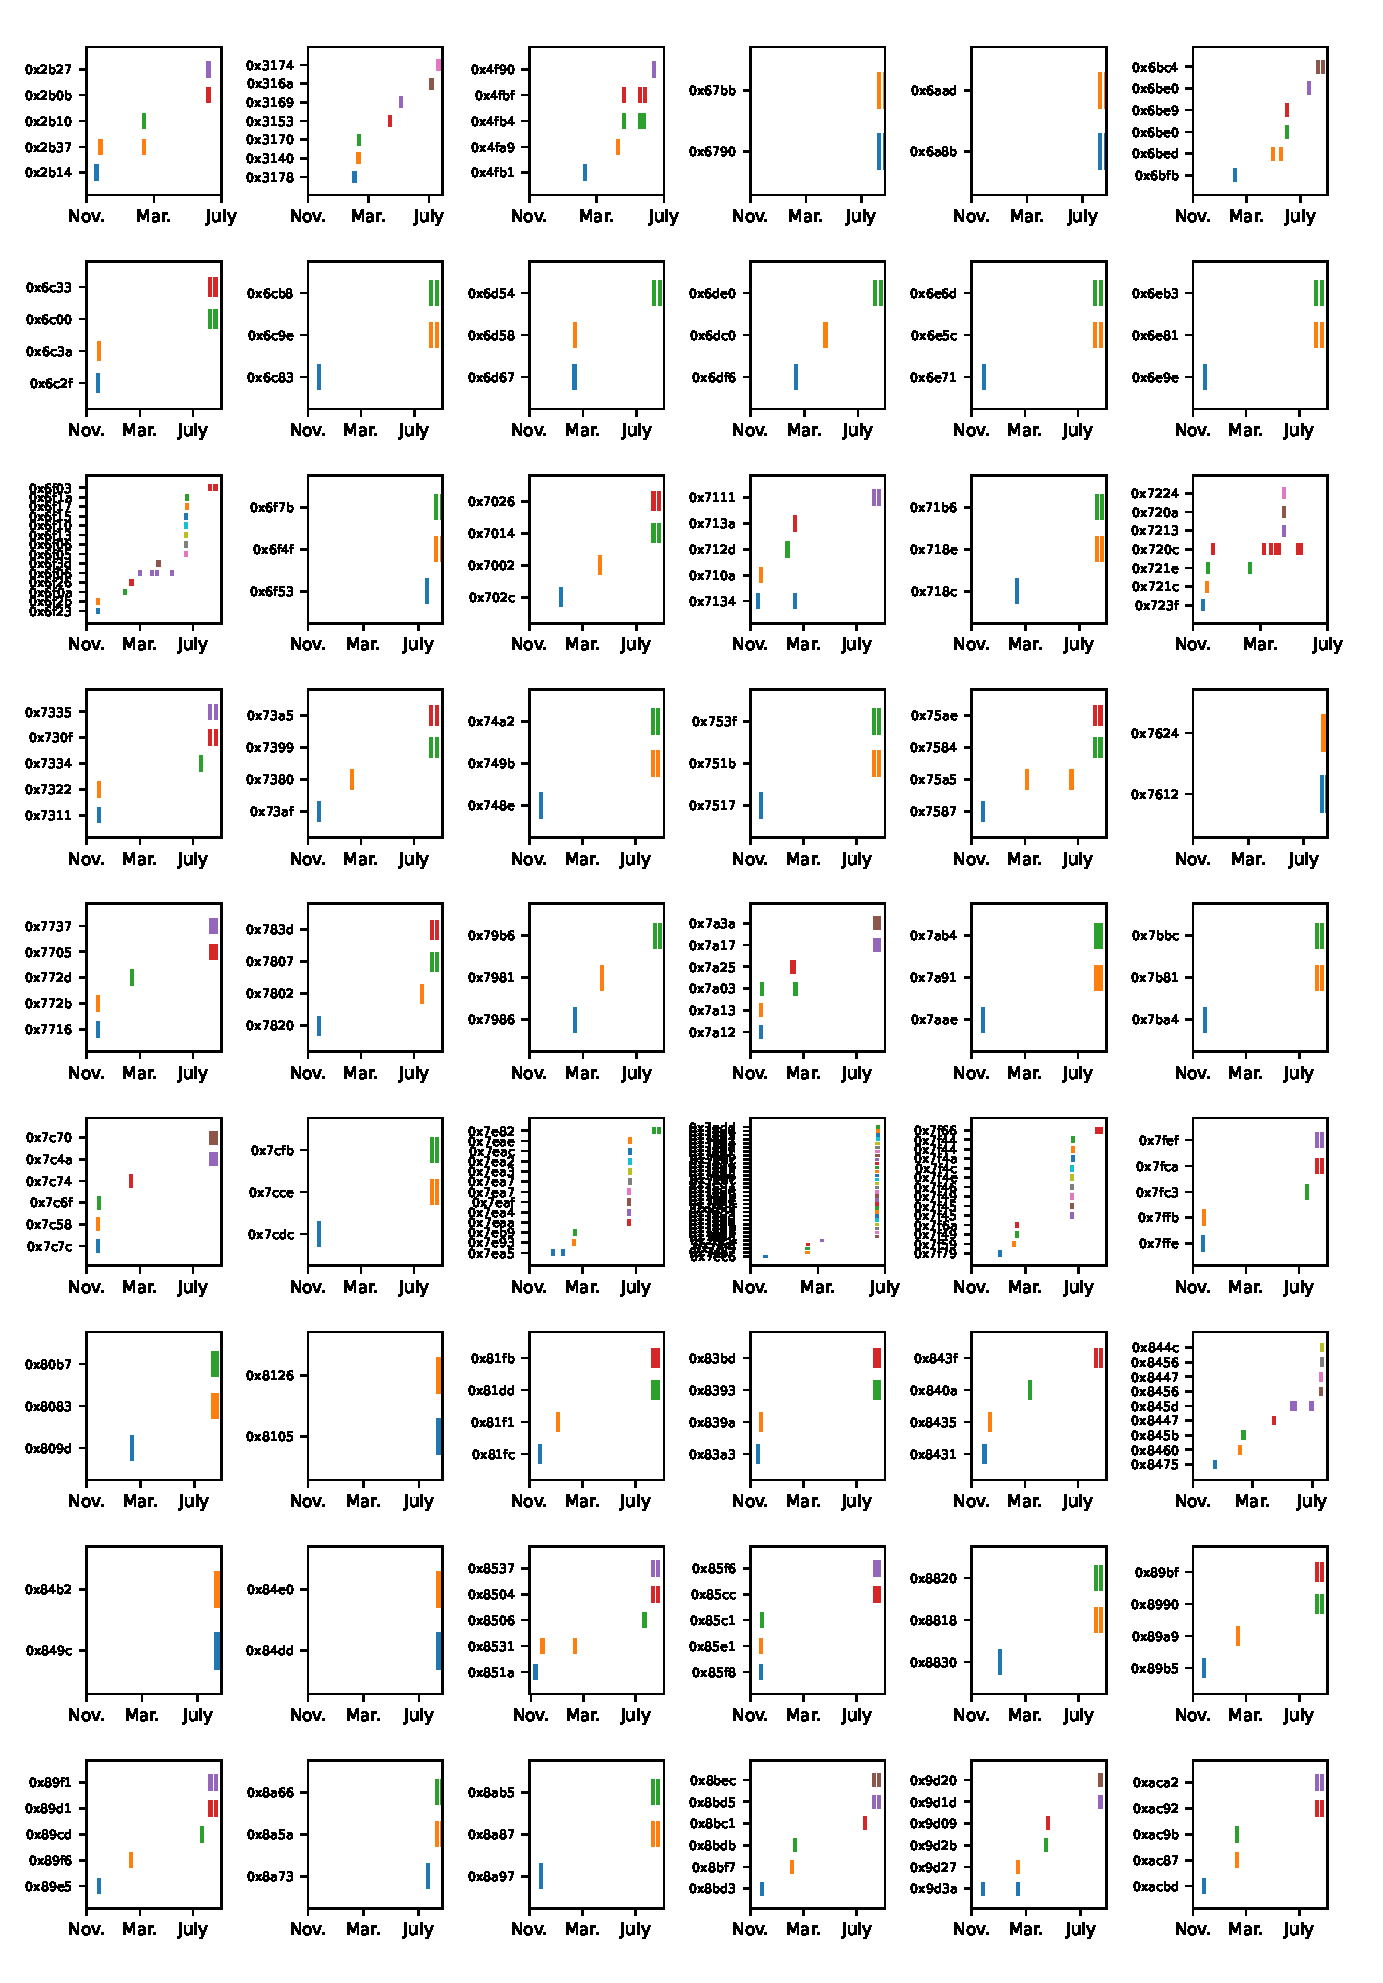
\includegraphics[width=\textwidth]{common/contested.eps}
%  \caption{Stake update events in contested neighbourhoods}
%  \label{event-plot}
%\end{figure}
%\end{center}


On many of the plots we can observe pairs of addresses that repeatedly top up at very similar times to one another.
%
We reproduce an example listing in Table \ref{event-listing}.
%
\begin{table}
\begin{tabular}{llr}
Date + time         & Address & Amount (BZZ) \\
\hline
2023-11-21 19:40:00 & 0x6c83 &   11 \\
2024-07-23 22:15:50 &	0x6c9e  &	10 \\
2024-07-23 22:16:05 &	0x6cb8  &	10 \\
2024-08-04 21:56:25 &	0x6c9e  &	10 \\
2024-08-04 21:56:45 &	0x6cb8  &	10
\end{tabular}
\caption{Event listing from in bin \code{0x6c8} --- cf.~the eighth plot in Figure \ref{event-plot}}
\label{event-listing}
\end{table}
%
We posit that the most likely reason for this behaviour is that the same entity started numerous nodes at the same time and placed them in distinct 11-bit neighbourhoods.
%
Since we have sorted by 10-bit neighbourhoods we have caught multiple of these nodes in the same bin, making their activity look like contention.


\appendix

\section{Notation index}

\paragraph{Addresses}

The set of agents is denoted $\Overlay$.
%
It can be realised as a set of \emph{overlay addresses}, for example, $\Overlay \cong \mathbb{F}_2^{256}$.

The set of overlay addresses is divided into a set $\Bins$ of \emph{bins}.
%
In \cite{book-of-swarm}, these are also called \emph{neighbourhoods}; we prefer the term `bins' because it is shorter and because neighbourhoods can also be of various different sizes.
%
We are given a surjective map $\bin:\Overlay\rightarrow\Bins$ that takes an overlay address to the bin to which it belongs.
%
The fibre of $\bin$ over a bin $\nu\in\Bins$ is denoted $\Overlay_\nu$.

In deployments, we have $\Bins\cong \mathbb{F}_2^D$ and the function $\bin$ is projection on the first $D$ bits, where $D$ is a network-wide dynamic variable called the \emph{network (log-)radius}.
%
For any $\nu\in\Bins$, we can then identify $\Overlay_\nu\simeq\mathbb{F}_2^{256-D}$ by projecting out the first $D$ bits.


\paragraph{Balances} Balances are presumed to be non-negative real numbers, i.e.~elements of $\uR := [0,\infty)$.

\paragraph{Summation}
Fix the following notation for summation over subsets of indices:
\begin{itemize}
  \item if $x\in \mathbb{R}^I$ is a vector of finite length, write $\sum:=\sum_I:\R^I\rightarrow\R$ for the sum of the coordinates. On $\uR^I$ this coincides with the 1-norm.
  \item If $J\subseteq I$ is a subset, write $\sum_J$ for the composite $\R^I\stackrel{\pi_J}{\rightarrow}\R^J\stackrel{\sum}{\rightarrow}\R$, that is, summation over the coordinates in $J$.
  \item If $i\in I$ is a single element, write also $\sum_{\hat{i}}$ as a shorthand for $\sum_{I\setminus\{i\}}$.
  \item If $M\leq N$ are natural numbers and $x\in\R^{\Overlay\times N}$, write $x_{\leq M}\in \uR^{\Overlay\times M}$ for the projection on the first $M$ terms.
\end{itemize}


\section{Ruin calculations}

\begin{lemma}

  $\sum_{n=N}^\infty { n\choose k } x^n = {k+N \choose k} \frac{x^N}{(1-x)^{N+k+1}}$

\end{lemma}

Summing over all integer hitting times and starting capital, we find
\begin{align*}
  \sum_{k=1}^\infty\sum_{n\in\N} \Prob[T_0 = n\mid C_0=k]u^k &= \sum_{k\in\N}\sum_{n\in\N} \frac{k}{n} \Prob[C_n = 0\mid C_0=k]u^k 
\end{align*}
\begin{align*}
  &= \sum_{k\in\N}\sum_{n\in\N} \frac{k}{n} \Prob[k - n + R\tilde{U}_n = 0]u^k \\
  &= \sum_{\ell\in\N}\sum_{n=\ell R}^\infty \frac{n-\ell R}{n} \Prob[\tilde{U}_n = \ell]u^{n-\ell R}   \qquad (k=n-\ell R)\\
  &= \sum_{\ell\in\N} \left( \frac{p}{qu^R} \right)^\ell \sum_{n=\ell R}^\infty \left[ 
    {n\choose \ell} - R \frac{\ell}{n} {n\choose \ell} 
  \right](uq)^n \\
  &= \sum_{\ell\in\N} \left( \frac{p}{qu^R} \right)^\ell 
  \left( 
    \sum_{n=\ell R}^\infty {n\choose \ell} (uq)^n - 
    Ruq \sum_{n=\ell R - 1}^\infty {n\choose \ell-1} (uq)^n
  \right) \\
  &= \sum_{\ell\in\N} \left( 
    \frac{p}{qu^R} 
  \right)^\ell 
  \left(
    {\ell(R+1) \choose \ell} \frac{ (uq)^{\ell R} } {(1-uq)^{\ell(R+1)+1} } - 
    Ruq {\ell(R+1)-2 \choose \ell - 1} \frac { (uq)^{\ell R-1} } { (1-uq)^{\ell(R+1) -1} }
  \right) \\
  &= \sum_{\ell\in\N} \left( 
    \frac{p(uq)^R}{qu^R(1-uq)^{R+1}} 
  \right)^\ell 
  \left(
    {\ell(R+1) \choose \ell} (1-uq)^{-1} - 
    R {\ell(R+1)-2 \choose \ell - 1} (1-uq)
  \right)  \\
  &= \sum_{\ell\in\N} \left( 
    \frac{pq^{R-1}}{(1-uq)^{R+1}} 
  \right)^\ell 
  \left(
    {\ell(R+1) \choose \ell} (1-uq)^{-1} - 
    R {\ell(R+1)-2 \choose \ell - 1} (1-uq)
  \right)
\end{align*}

We don't know a closed form for the series $\sum_\ell { k\ell \choose \ell }x^\ell $ for general $k>2$.
%
However, for $k=2$ the coefficients are the central binomial coefficients, which we can study in closed form (although this case $R=1$ is not very important in practice).
%
\begin{align*}
  &= \sum_{\ell\in\N} \left( 
    \frac{p}{(1-uq)^{2}} 
  \right)^\ell 
  \left(
    {2\ell \choose \ell} (1-uq)^{-1} - 
    R {2(\ell-1) \choose \ell - 1} (1-uq)
  \right) \\
  &= \sum_{\ell\in\N} \left( 
    \frac{p}{(1-uq)^{2}} 
  \right)^\ell 
  \left(
    {2\ell \choose \ell} \frac{1-Rp}{1-uq}
  \right) \\
  &= \frac{1-Rp}{1-uq}\left(
    1 - 4\cdot \frac{p}{(1-uq)^{2}}
  \right)^{-\frac{1}{2}} 
\end{align*}

To solve for the eventual ruin probability, we need to specialise to fixed $k>0$ and sum over $n\in\N$.
%
In principle, we can extract this from the generating function by applying $\frac{\partial^k}{k!\partial u^k}$ and evaluating at $u=0$.
%
However, without any clear sign this is going to produce anything userful, we put aside the effort.

%\begin{align*}
%  \sum_{k\in\N}\sum_{n\in\N} \Prob[T_0 = n\mid C_0=k]u^k &= \left( 1- \frac{pu^{-R}}{(1-p)(1-u(1-p))} \right)^{-1}((1-u(1-p))^{-1}-R) 
%\end{align*}
%Then applying the $k$th derivative, we get


%?
%\[
%  \Prob(T_0 <\infty\mid C_0=k) = (1-p)^{-k}(p^{-1}-R)
%\]